\documentclass[11pt,a4paper]{article}
\usepackage[utf8]{inputenc}
\usepackage[T1]{fontenc}
\usepackage[polish]{babel}
\usepackage{lmodern}
\usepackage{microtype}
\usepackage[a4paper,margin=2.3cm]{geometry}
\usepackage{amsmath,amssymb}
\usepackage{booktabs,multirow,tabularx,array}
\usepackage{graphicx}
\usepackage{float}
\usepackage[font=small,labelfont=bf]{caption}
\usepackage{subcaption}
\usepackage{enumitem}
\usepackage{xcolor}
\usepackage[locale=DE,group-minimum-digits=4]{siunitx}
\usepackage{listings}
\usepackage[hidelinks]{hyperref}

\definecolor{accent}{HTML}{2a78d6}
\definecolor{codebg}{HTML}{f4f4f2}
\lstset{basicstyle=\ttfamily\footnotesize,backgroundcolor=\color{codebg},frame=none,
  columns=fullflexible,breaklines=true,xleftmargin=4pt,aboveskip=6pt,belowskip=6pt}
\setlist{itemsep=2pt,topsep=4pt}
\graphicspath{{figures/}{../EDA/figures/}}
\newcommand{\code}[1]{\texttt{#1}}
\makeatletter\newcommand{\tabinput}[1]{\@@input #1 }\makeatother
\renewcommand{\arraystretch}{1.12}

\title{\textbf{Biometryczna weryfikacja użytkowników VR\\na podstawie ruchu w scenariuszu cross-day}\\[4pt]
\large Raport techniczny -- Deep Learning w Biometrii, spotkania \#1--3}
\author{Dominik Zabielski \and Hubert Żochowski \and Michał Dąbrowski}
\date{24 listopada 2026}

\begin{document}
\maketitle

\begin{abstract}
\noindent
Badamy identyfikację i weryfikację 41 osób na podstawie trajektorii hełmu i dwóch kontrolerów VR
podczas rzutu piłką do kosza (korpus VR-Biometric-Authentication, 3 zestawy: Quest, Vive, Cosmos).
Modele uczymy na nagraniach z dnia~1, a oceniamy na nagraniach z dnia~2 (cross-day), porównując
embeddingi podobieństwem cosinusowym (Rank-1, Rank-5, EER). Wytrenowaliśmy trzy klasyfikatory z listy
-- ResNet1D, GRU i Transformer -- oraz przeprowadziliśmy ablację modalności (pozycja / rotacja / pełny
zbiór) na trzech ziarnach losowania i analizę RSA reprezentacji. Kluczowe dla jakości okazało się
poprawne kodowanie rotacji: surowe kąty Eulera zastąpiliśmy ciągłą reprezentacją 6D, co odwróciło
wnioski ablacji -- rotacja niesie więcej informacji biometrycznej niż pozycja. W scenariuszu bazowym
najlepszy jest Transformer (Rank-1 $0{,}938 \pm 0{,}017$ na dniu~2). W scenariuszu rozszerzonym
(ArcFace, augmentacje, EMA, cechy odporne na zmianę dnia, czwarty model InceptionTime i ensemble)
ensemble czterech modeli osiąga Rank-1 $0{,}977 \pm 0{,}002$ i EER $0{,}012$ na odłożonej połowie
dnia~2, której nie używaliśmy do żadnej decyzji; na całym dniu~2 to 0{,}985 i 0{,}009. Oznacza to
ok.~4 razy mniej błędów identyfikacji niż w najlepszym modelu bazowym. Najbardziej informatywny
biometrycznie jest zestaw Quest, najmniej -- Cosmos.

\end{abstract}

\tableofcontents
\newpage

%=====================================================================
\section{Cel i zakres}
%=====================================================================
Celem jest sprawdzenie, czy sposób wykonywania prostego zadania ruchowego w wirtualnej rzeczywistości
pozwala rozpoznać osobę \emph{innego dnia} niż dzień rejestracji. Tabela~\ref{tab:mapa} wiąże punkty
polecenia z sekcjami raportu.

\begin{table}[H]
\centering\small
\caption{Punkty polecenia a zawartość raportu.}
\label{tab:mapa}
\begin{tabularx}{\linewidth}{@{}lXl@{}}
\toprule
\# & Wymaganie z polecenia & Sekcja \\
\midrule
1 & Eksploracyjna analiza danych (EDA) & \ref{sec:eda} \\
2 & Weryfikacja cross-day: trening na dniu 1, test na dniu 2 & \ref{sec:protokol}, \ref{sec:wyniki-s1} \\
3 & Trzy klasyfikatory z listy (wybrano ResNet, GRU, Transformer; dodatkowo InceptionTime) & \ref{sec:modele} \\
4 & Ocena: Rank-1 i podobieństwo cosinusowe (dodatkowo Rank-5, EER, krzywe CMC i DET) & \ref{sec:ewaluacja}, \ref{sec:wyniki} \\
5 & Ablacja: pozycja / kąty obrotu / pełny zbiór & \ref{sec:wyniki-s2} \\
6 & RSA embeddingów, wnioski o urządzeniach i modelach & \ref{sec:wyniki-s3}, \ref{sec:wnioski} \\
-- & Zapis \code{train\_embedding.npz} i \code{test\_embedding.npz} & \ref{sec:odtwarzalnosc} \\
\bottomrule
\end{tabularx}
\end{table}

%=====================================================================
\section{Korpus danych i analiza eksploracyjna}\label{sec:eda}
%=====================================================================
\subsection{Charakterystyka zbioru}
Korpus VR-Biometric-Authentication \cite{dataset} zawiera nagrania 41 uczestników wykonujących
w VR rzut piłką do kosza. Każda osoba wykonała
po 10 rzutów na każdym z trzech zestawów (Meta Quest, HTC Vive, HTC Vive Cosmos) w dwóch dniach. Dane
są zapisane jako 6 sesji (urządzenie $\times$ dzień) o kształcie $(41, 10, 135, 21)$: osoba, rzut,
135 kroków czasowych i 21 kanałów. Kanały to trzy grupy po 7 cech -- prawy kontroler, hełm, lewy
kontroler -- a w każdej grupie: pozycja $(x, y, z)$, kąty Eulera $(r_x, r_y, r_z)$ i stan spustu.
Oś $y$ jest pionowa (wysokość hełmu ok.~2{,}07 w jednostkach sceny).

\begin{itemize}
  \item \textbf{Kompletność:} brak wartości NaN i nieskończonych, brak pustych sesji; wszystkie pliki
        mają identyczny kształt.
  \item \textbf{Rozkład klas:} idealnie zbalansowany -- 30 próbek na osobę i dzień (3 urządzenia
        $\times$ 10 rzutów), 410 próbek na urządzenie i dzień; łącznie 1230 próbek na dzień i 2460
        w całym korpusie (rys.~\ref{fig:eda-klasy}).
  \item \textbf{Kanały nieinformatywne:} spust hełmu jest stale równy zero, spust lewego kontrolera
        prawie zawsze zero, a spust prawego kontrolera to sygnał binarny wyrzutu. Do modeli
        używamy więc tylko pozycji i rotacji (18 kanałów surowych).
  \item \textbf{Wartości odstające} (kryterium $1{,}5\cdot$IQR per kanał): obecne we wszystkich
        sesjach, najwięcej w sesjach Vive (ok.~25~tys. wartości wobec 13--15~tys. dla pozostałych
        zestawów); pojedyncze skrajne pozycje (np. $x=-10{,}6$) wskazują na chwilową utratę śledzenia.
        Nie usuwamy ich -- normalizacja $z$-score jest liczona na całym dniu~1, a modele z
        normalizacją wsadową i uśrednianiem w czasie okazały się na nie odporne.
\end{itemize}

\begin{figure}[H]
\centering
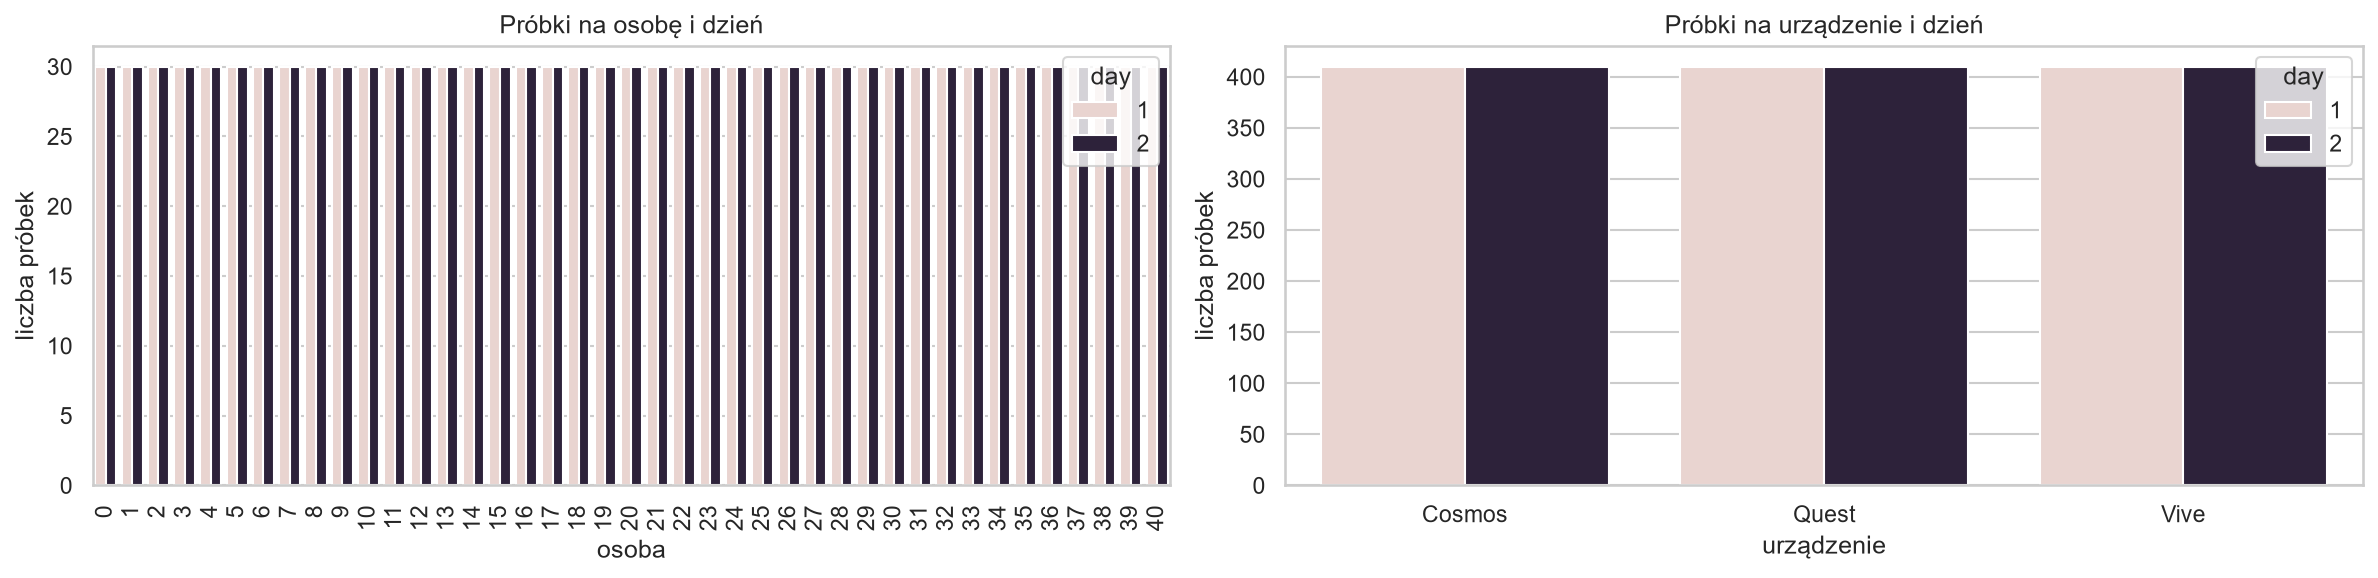
\includegraphics[width=0.75\linewidth]{rozklad_klas.png}
\caption{Rozkład próbek na osoby i urządzenia (EDA) -- korpus jest idealnie zbalansowany.}
\label{fig:eda-klasy}
\end{figure}

\subsection{Trajektorie, zmienność między osobami i między dniami}
Rzut ma powtarzalną strukturę: zamach (wzniesienie kontrolera), wyrzut ok.~60. kroku i powrót
(rys.~\ref{fig:eda-traj}). Kształt trajektorii tej samej osoby jest bardzo zbliżony między dniami,
natomiast między osobami różni się amplituda, tempo i moment wyrzutu -- to właśnie ta zmienność
niesie informację biometryczną. Średnie kanałów między dniami są prawie identyczne (różnice rzędu
0{,}01), ale zmieniają się wariancje i liczba wartości odstających, a różne zestawy mają wyraźnie
różne odchylenia standardowe rotacji (rys.~\ref{fig:eda-urz}). Walidacja w obrębie dnia~1 jest więc
optymistyczna, a jedyną miarodajną oceną jest dzień~2.

\begin{figure}[H]
\centering
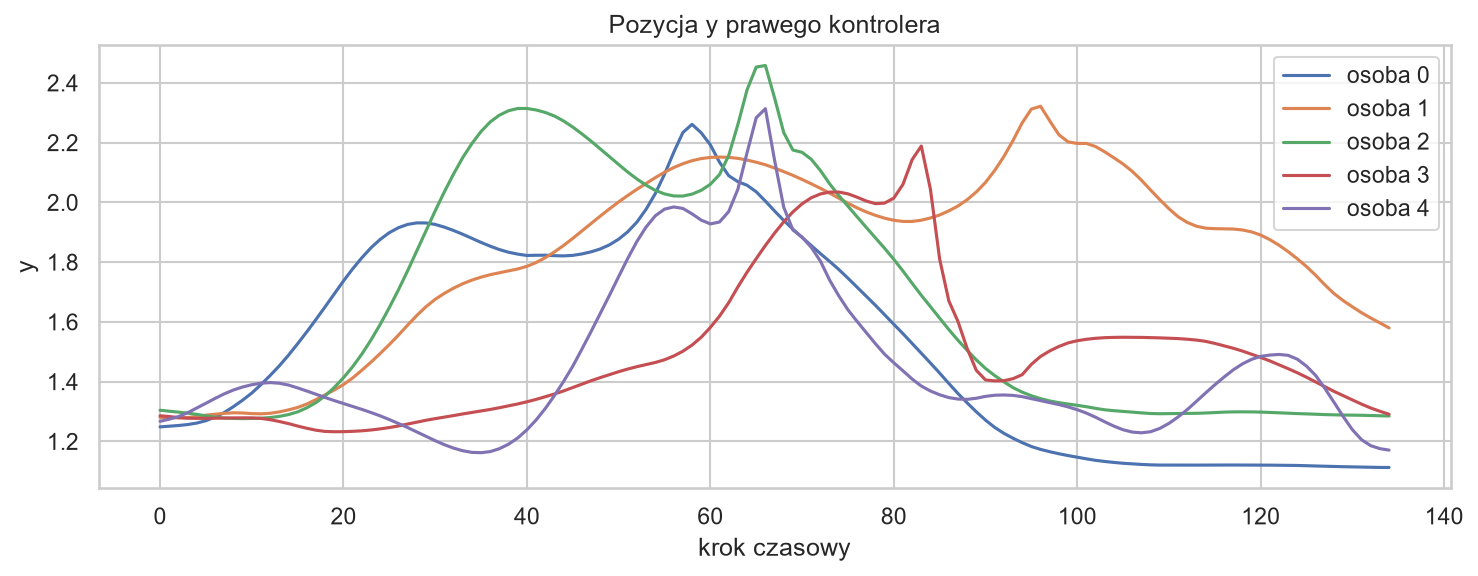
\includegraphics[height=3.6cm]{zmiennosc_miedzyosobnicza.png}\\[2pt]
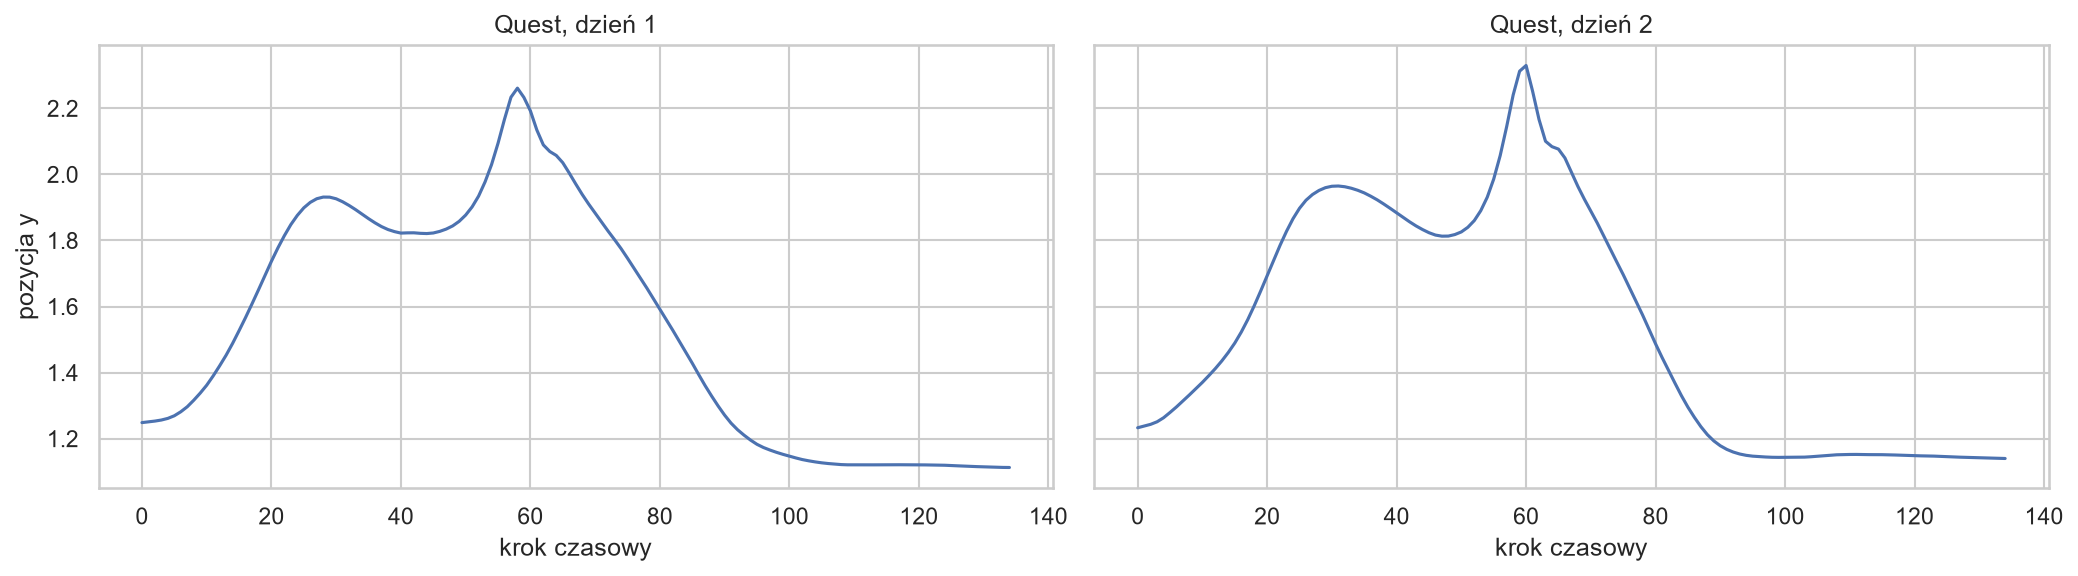
\includegraphics[height=3.6cm]{trajektorie_dzien1_dzien2.png}
\caption{Góra: pozycja $y$ prawego kontrolera dla 5 osób (zmienność międzyosobnicza).
Dół: ta sama osoba i urządzenie w dniu 1 i 2 -- kształt rzutu jest stabilny.}
\label{fig:eda-traj}
\end{figure}

\begin{figure}[H]
\centering
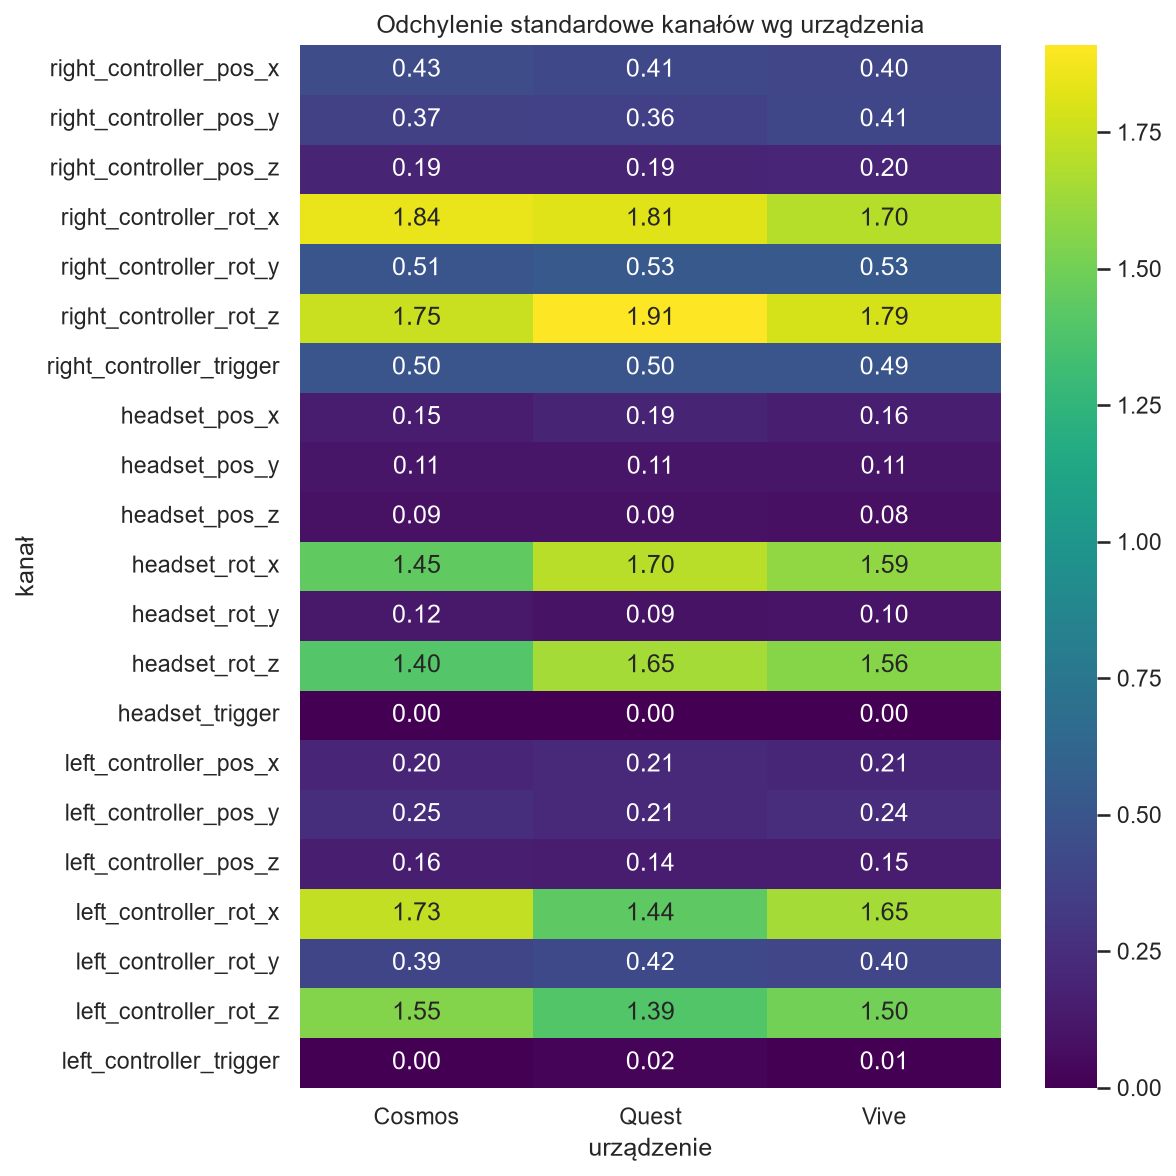
\includegraphics[width=0.5\linewidth]{odchylenia_urzadzenia.png}
\caption{Odchylenie standardowe kanałów w podziale na urządzenia (EDA).}
\label{fig:eda-urz}
\end{figure}

\subsection{Nieciągłość kątów Eulera i reprezentacja 6D}\label{sec:rot6d}
Najważniejsze odkrycie EDA dotyczy rotacji. Kąty Eulera są nieciągłe: zawijają się na granicy
$\pm\pi$, a przy $r_y \approx -\pi/2$ występuje \emph{gimbal lock}, gdy $r_x$ i $r_z$ przeskakują
razem, mimo że sama orientacja zmienia się płynnie. Skok większy niż 1~rad między sąsiednimi
klatkami występuje w 90\% nagrań prawego kontrolera, 29\% nagrań hełmu i 13\% nagrań lewego
kontrolera. Takie skoki są dla sieci artefaktem nie do odróżnienia od ruchu.

Dlatego kąty zamieniamy na macierz rotacji $R \in SO(3)$ (kolejność \code{xyz}) i używamy jej dwóch
pierwszych kolumn -- ciągłej reprezentacji 6D \cite{zhou6d}. Po tej zmianie ruch hełmu i lewego
kontrolera jest w pełni płynny (0\% nagrań ze skokiem); u prawego kontrolera skok pozostaje w 48\%
nagrań dokładnie w momencie wyrzutu, czyli wynika z rzeczywistego, szybkiego obrotu nadgarstka
(rys.~\ref{fig:eda-rot}). Wejście modelu ma 27 kanałów: 9 pozycji i $3 \times 6 = 18$ cech rotacji.

\begin{figure}[H]
\centering
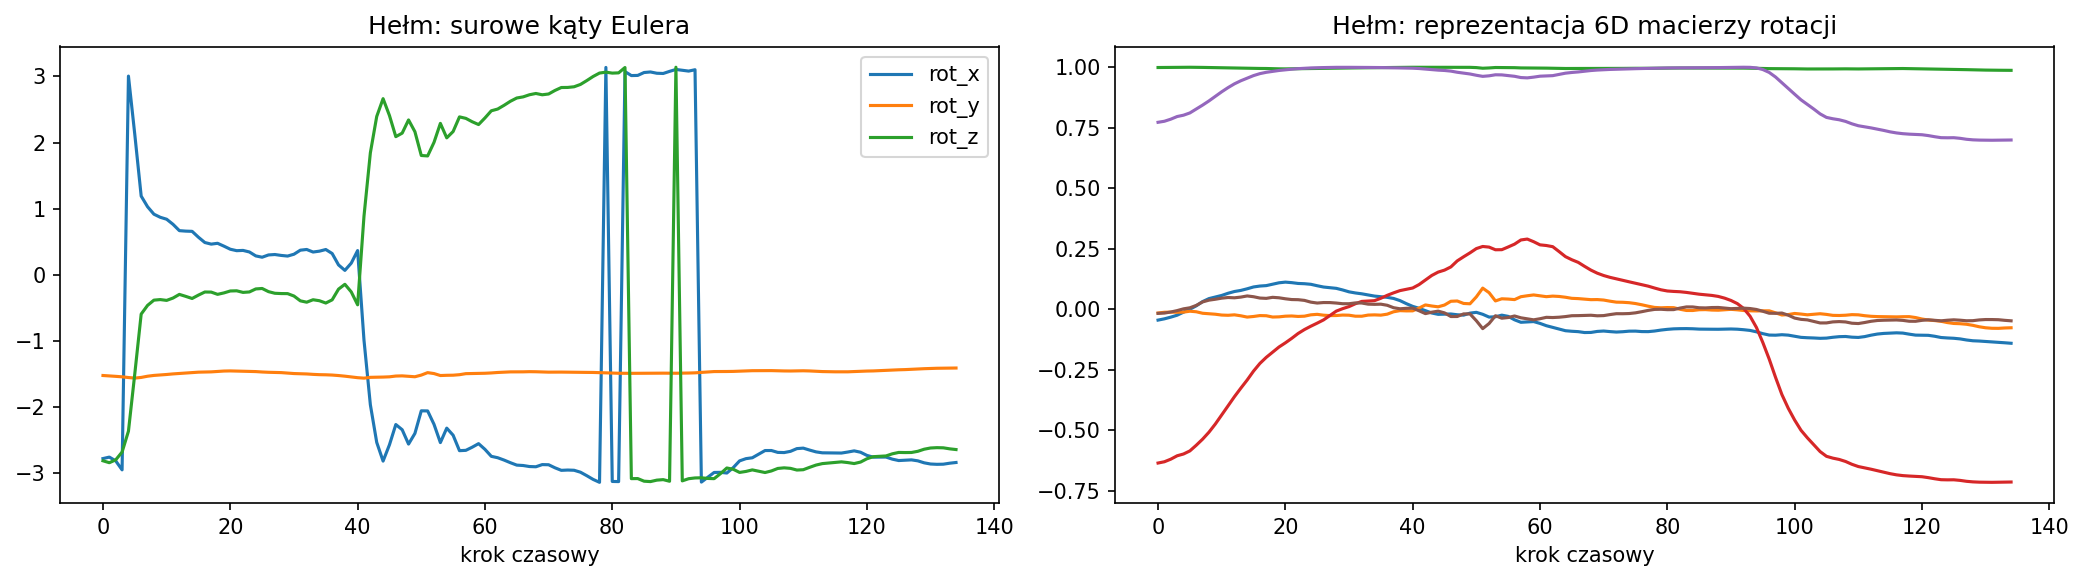
\includegraphics[width=\linewidth]{rotacja_euler_vs_6d.png}
\caption{Ten sam rzut: surowe kąty Eulera hełmu (lewo, skoki o $2\pi$ i gimbal lock) oraz
reprezentacja 6D macierzy rotacji (prawo, przebieg ciągły).}
\label{fig:eda-rot}
\end{figure}

%=====================================================================
\section{Metodyka}
%=====================================================================
\subsection{Protokół cross-day}\label{sec:protokol}
\begin{itemize}
  \item \textbf{Trening:} dzień 1, wszystkie urządzenia (1230 próbek). Z dnia~1 wydzielamy walidację
        stratyfikowaną po parach (osoba, urządzenie): 2 losowe rzuty z każdej z $41 \times 3 = 123$
        grup, czyli 984 próbki treningowe i 246 walidacyjnych. Każda osoba i każde urządzenie są
        reprezentowane w walidacji.
  \item \textbf{Test:} dzień 2 (1230 próbek), nieużywany w żaden sposób podczas treningu ani doboru
        hiperparametrów w scenariuszach S1--S3.
  \item \textbf{Normalizacja:} $z$-score per kanał ze statystykami dnia~1 (te same parametry
        stosujemy do dnia~2).
  \item \textbf{Identyfikacja i weryfikacja:} galerią są embeddingi próbek treningowych dnia~1,
        próbami (\emph{probe}) -- embeddingi dnia~2. Klasyfikator służy wyłącznie do nauczenia
        przestrzeni embeddingów; decyzje biometryczne podejmujemy na podobieństwie cosinusowym.
\end{itemize}

\subsection{Modele}\label{sec:modele}
Wybraliśmy trzy modele z trzech \emph{różnych} kategorii z listy, aby porównać różne założenia
indukcyjne: konwolucyjne (lokalne wzorce), rekurencyjne (dynamika sekwencyjna) i oparte na uwadze
(globalny kontekst). Każdy zwraca parę (logity, embedding); embedding to wyjście warstwy
\code{Linear} po globalnym uśrednieniu cech w czasie.
\begin{itemize}
  \item \textbf{ResNet1D} \cite{resnet} -- splot 1D (jądro 7) i 3 etapy po 2 bloki rezydualne
        (jądro 3, BatchNorm, ReLU, dropout), podwajanie kanałów i stride 2 na etap, globalne
        uśrednianie. Dobrze wychwytuje lokalne wzorce: przyspieszenia, zmiany kierunku, moment
        wyrzutu; połączenia rezydualne stabilizują trening.
  \item \textbf{GRU} \cite{gru} -- dwukierunkowa sieć GRU z uśrednianiem stanów w czasie. Modeluje
        kolejność zdarzeń przy małej liczbie parametrów i jest lżejsza od LSTM przy podobnej sile na
        krótkich sekwencjach (135 kroków).
  \item \textbf{Transformer} \cite{transformer} -- rzut liniowy do $d_\text{model}$, sinusoidalne
        kodowanie pozycji, enkoder pre-LN z aktywacją GELU, uśrednianie tokenów. Self-attention łączy
        odległe fragmenty rzutu (zamach z wyrzutem) bez ograniczeń pola recepcyjnego.
  \item \textbf{InceptionTime} \cite{inceptiontime} (tylko w scenariuszu S4) -- 6 modułów Inception
        (bottleneck $1\times1$, równoległe sploty o jądrach 39/19/9 i gałąź max-pool, 128 kanałów
        wyjściowych), połączenia rezydualne co 3 moduły. Jest uznanym punktem odniesienia w
        klasyfikacji szeregów czasowych, więc dodaliśmy go jako czwarty model z listy.
\end{itemize}

\subsection{Trening i dobór hiperparametrów}\label{sec:trening}
Wspólne ustawienia (S1--S3): entropia krzyżowa z wygładzaniem etykiet 0{,}05, optymalizator AdamW
\cite{adamw}, harmonogram cosinusowy, przycinanie normy gradientu do 1, maks. 60 epok. Model
wybieramy po minimalnym \emph{val loss} z cierpliwością 12 epok. Val Rank-1 z dnia~1 szybko dochodzi
do ok.~1{,}0 i przestaje rozróżniać modele, dlatego nie nadaje się na kryterium.

Hiperparametry dobraliśmy \textbf{random search} \cite{randomsearch} (6 prób $\times$ 15 epok na
model, wybór po val loss): lr $\in [2\cdot10^{-4}, 3\cdot10^{-3}]$ (log), weight decay
$\in [10^{-4}, 2\cdot10^{-2}]$ (log), batch $\in \{32, 64\}$, dropout, wymiar embeddingu
$\in \{64, 128, 256\}$ oraz parametry architektury. Grid search rośnie wykładniczo z liczbą
parametrów, a random search przy tym samym budżecie lepiej pokrywa wymiary istotne. Wybrane
konfiguracje zawiera tabela~\ref{tab:hparams}.

\begin{table}[H]
\centering\small
\caption{Hiperparametry wybrane przez random search (modalność pełna).}
\label{tab:hparams}
\setlength{\tabcolsep}{4pt}
\begin{tabularx}{\linewidth}{@{}l>{\raggedright\arraybackslash}Xrrrrrr@{}}
\toprule
Model & Architektura & Emb. & Dropout & lr & wd & Batch & Parametry \\
\midrule
\tabinput{tables/hparams.tex}
\bottomrule
\end{tabularx}
\end{table}

\subsection{Metryki ewaluacji}\label{sec:ewaluacja}
Dla probe $q$ i próbki galerii $g$ podobieństwo to $s(q,g) = \frac{q^\top g}{\|q\|\|g\|}$.
\begin{itemize}
  \item \textbf{Rank-$k$ (identyfikacja, zbiór zamknięty):} wynik osoby $c$ to
        $S_c(q) = \max_{g:\, y_g = c} s(q, g)$; trafienie, gdy prawdziwa osoba jest wśród $k$ osób o
        najwyższym $S_c$. Ranking jest po \emph{osobach}, a nie po próbkach -- inaczej $k$
        najbliższych próbek mogłoby należeć do jednej osoby i Rank-5 byłby sztucznie równy Rank-1.
        Rank-1 raportujemy też osobno dla prób z każdego urządzenia.
  \item \textbf{Podobieństwo cosinusowe genuine / impostor:} średnie $s(q,g)$ dla par tej samej
        osoby i par różnych osób; im większa różnica, tym lepsza separacja.
  \item \textbf{EER (weryfikacja):} na wszystkich parach (probe, galeria) wyznaczamy FAR
        (odsetek par impostor powyżej progu) i FRR (odsetek par genuine poniżej progu); EER to
        punkt, w którym FAR $=$ FRR. Pokazujemy też krzywe CMC (Rank-$k$ dla $k=1..10$) i DET.
\end{itemize}

%=====================================================================
\section{Scenariusze badawcze}
%=====================================================================
\begin{table}[H]
\centering\small
\caption{Badane scenariusze.}
\label{tab:scenariusze}
\begin{tabularx}{\linewidth}{@{}lXl@{}}
\toprule
Scenariusz & Konfiguracja & Wynik \\
\midrule
S1 -- główny cross-day & 3 modele, modalność pełna, seed 42, hiperparametry z random search & tab.~\ref{tab:main} \\
S2 -- ablacja modalności & 3 modele $\times$ \{pozycja, rotacja 6D, pełny\} $\times$ 3 seedy (42, 43, 44); hiperparametry ze strojenia na pełnym zbiorze; seed zmienia inicjalizację, kolejność batchy i podział walidacji & tab.~\ref{tab:ablation} \\
S3 -- RSA & RDM $= 1 - \cos$ między wszystkimi parami 1230 prób dnia~2 dla 9 przebiegów z S2 (seed 42); korelacja Spearmana RDM model--model oraz z RDM tożsamości i urządzenia & tab.~\ref{tab:rsa} \\
S4 -- rozszerzony (SOTA) & ArcFace, augmentacje, EMA, cechy odporne na zmianę dnia, InceptionTime, ensemble; wybór przepisu na połowie dnia~2 (\emph{dev}), raport na drugiej połowie (\emph{test}) & sek.~\ref{sec:sota} \\
\bottomrule
\end{tabularx}
\end{table}

%=====================================================================
\section{Wyniki}\label{sec:wyniki}
%=====================================================================
\subsection{S1: główny eksperyment cross-day}\label{sec:wyniki-s1}

\begin{table}[H]
\centering\small
\setlength{\tabcolsep}{4.5pt}
\caption{S1: modalność pełna, seed 42. Val -- dzień 1 (wybór modelu), pozostałe kolumny -- dzień 2.}
\label{tab:main}
\begin{tabular}{@{}lrrrrrrrrrr@{}}
\toprule
& & & \multicolumn{3}{c}{Dzień 2} & \multicolumn{2}{c}{cos} & \multicolumn{3}{c}{Rank-1 wg urządzenia} \\
\cmidrule(lr){4-6}\cmidrule(lr){7-8}\cmidrule(l){9-11}
Model & Epoka & Val R-1 & Rank-1 & Rank-5 & EER & genuine & impostor & Quest & Vive & Cosmos \\
\midrule
\tabinput{tables/main.tex}
\bottomrule
\end{tabular}
\end{table}

Najlepszy jest Transformer (Rank-1 0{,}957, Rank-5 0{,}993), tuż za nim ResNet1D (0{,}932) z
najniższym EER (0{,}018). GRU wyraźnie odstaje (0{,}792). Spadek val~$\to$~test pokazuje koszt
zmiany dnia: dla GRU 0{,}97~$\to$~0{,}79, dla modeli konwolucyjnego i attention ok.~4--6 p.p.
Transformer najlepiej separuje osoby -- ma najniższe średnie podobieństwo impostor (0{,}28 wobec
0{,}47 dla ResNet1D), co widać na rozkładach wyników (rys.~\ref{fig:scores-base}). ResNet1D ma
wysokie podobieństwo genuine, ale też wysoko położony rozkład impostor, bo embedding po ReLU jest
nieujemny i zajmuje tylko część sfery.

\begin{figure}[H]
\centering
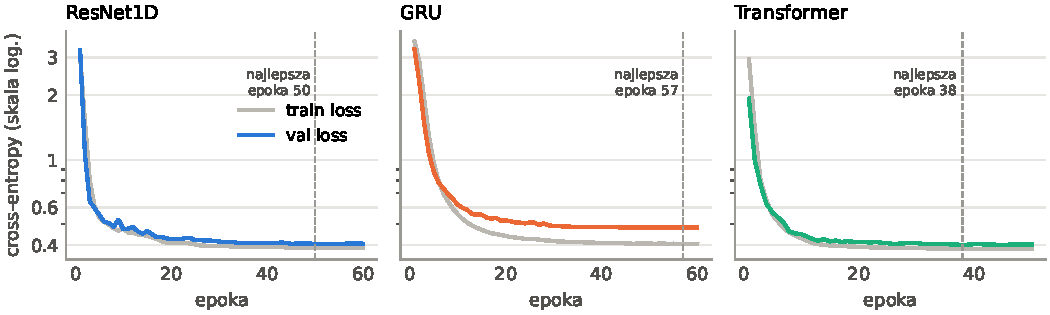
\includegraphics[width=\linewidth]{training_curves.pdf}
\caption{Krzywe uczenia (S1). Linia przerywana -- epoka wybrana po minimalnym val loss.}
\label{fig:curves}
\end{figure}

\begin{figure}[H]
\centering
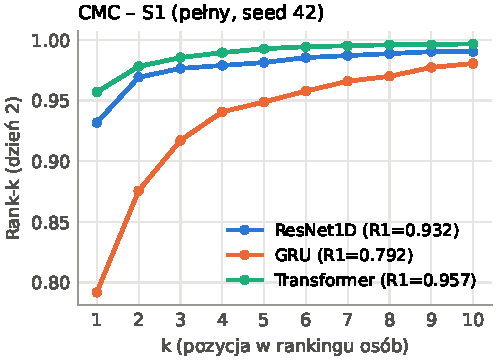
\includegraphics[width=0.55\linewidth]{cmc_baseline.pdf}
\caption{Krzywe CMC na dniu 2 (S1). Rank-3 wynosi 0{,}985 dla Transformera i 0{,}976 dla ResNet1D; GRU zyskuje najwięcej (Rank-1 0{,}79, Rank-3 0{,}92).}
\label{fig:cmc-base}
\end{figure}

\begin{figure}[H]
\centering
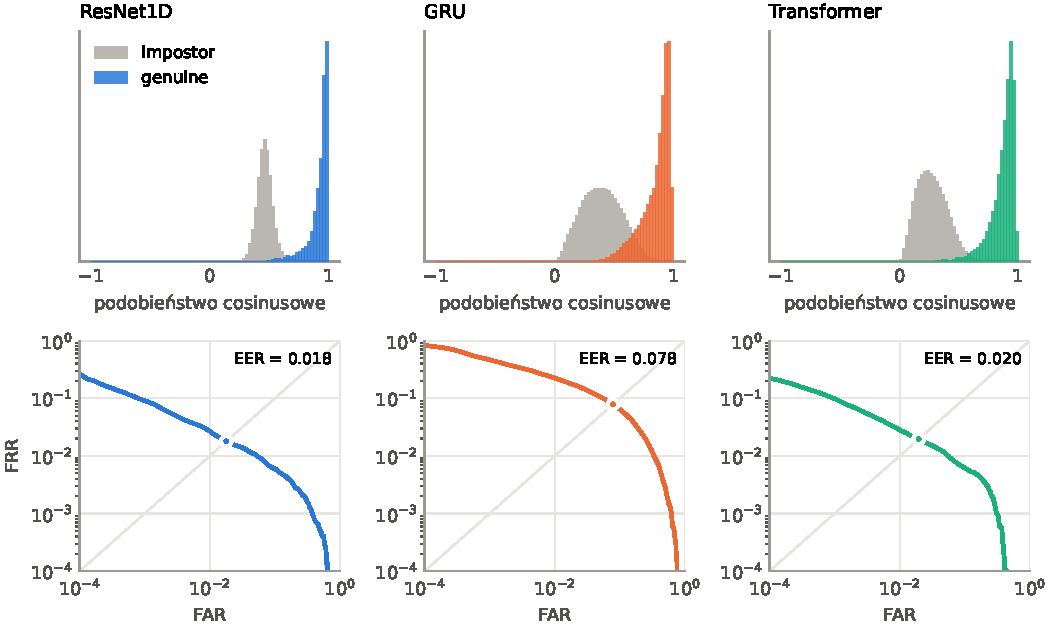
\includegraphics[width=\linewidth]{scores_baseline.pdf}
\caption{Góra: rozkłady podobieństwa cosinusowego par genuine i impostor (dzień 2 vs galeria
z dnia 1). Dół: krzywe DET (skala log.) z zaznaczonym EER.}
\label{fig:scores-base}
\end{figure}

\subsection{S2: ablacja modalności}\label{sec:wyniki-s2}

\begin{table}[H]
\centering\small
\setlength{\tabcolsep}{2.6pt}
\caption{S2: średnia $\pm$ odchylenie standardowe z 3 seedów (dzień 2). Pogrubienie -- najlepsza
modalność dla modelu.}
\label{tab:ablation}
\begin{tabular}{@{}llrrrrrrrr@{}}
\toprule
& & & & & \multicolumn{2}{c}{cos} & \multicolumn{3}{c}{Rank-1 wg urządzenia} \\
\cmidrule(lr){6-7}\cmidrule(l){8-10}
Model & Modalność & Rank-1 & Rank-5 & EER & gen. & imp. & Quest & Vive & Cosmos \\
\midrule
\tabinput{tables/ablation.tex}
\bottomrule
\end{tabular}
\end{table}

\begin{figure}[H]
\centering
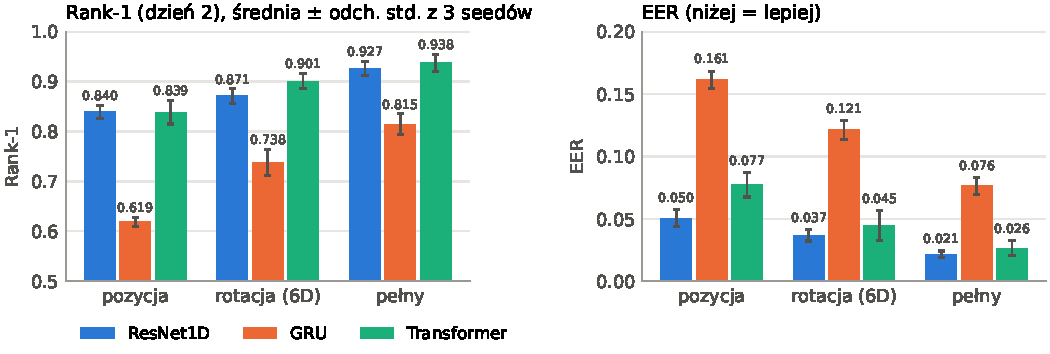
\includegraphics[width=\linewidth]{ablation_modality.pdf}
\caption{S2: Rank-1 i EER w zależności od modalności (średnia $\pm$ odch. std. z 3 seedów).}
\label{fig:ablation}
\end{figure}

\begin{itemize}
  \item \textbf{Pełny $>$ rotacja $>$ pozycja} dla \emph{każdego} modelu i każdej metryki (Rank-1,
        Rank-5, EER, RSA z tożsamością). Obie modalności są komplementarne -- pełny zbiór poprawia
        najlepszą pojedynczą modalność o 4--8 p.p. Rank-1.
  \item \textbf{Rotacja niesie więcej informacji niż pozycja}, np. GRU 0{,}738 vs 0{,}619,
        Transformer 0{,}901 vs 0{,}839. W pierwszej wersji projektu, na surowych kątach Eulera,
        wynik był \emph{odwrotny} (GRU: rotacja 0{,}522 vs pozycja 0{,}619; Transformer 0{,}767 vs
        0{,}888). Różnica wynika wyłącznie z reprezentacji (sek.~\ref{sec:rot6d}): orientacja
        dłoni i głowy jest silną cechą biometryczną, ale tylko w ciągłym kodowaniu.
  \item Różnice między seedami są małe (odch. std. Rank-1 0{,}01--0{,}03), więc ranking modalności i
        modeli jest stabilny.
\end{itemize}

\begin{figure}[H]
\centering
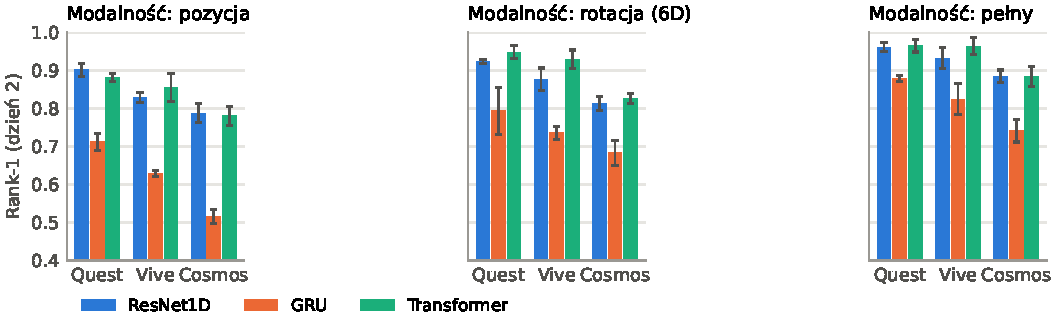
\includegraphics[width=\linewidth]{rank1_devices.pdf}
\caption{S2: Rank-1 w podziale na urządzenie, z którego pochodzi próba (średnia z 3 seedów).}
\label{fig:devices}
\end{figure}

\textbf{Urządzenia.} Cosmos ma najniższy Rank-1 we \emph{wszystkich} 9 konfiguracjach
(model~$\times$~modalność), a Quest -- najwyższy w 9 z 9 (dla Transformera na pełnym zbiorze to
praktycznie remis z Vive: 0{,}965 vs 0{,}964). Najbardziej informatywny biometrycznie okazuje się
więc Quest, najmniej -- Cosmos. Przewaga Questa jest największa dla samej pozycji, co sugeruje
stabilniejsze śledzenie pozycji między sesjami; jest to hipoteza, której ten korpus nie pozwala
rozstrzygnąć.

\subsection{S3: Representational Similarity Analysis}\label{sec:wyniki-s3}
Dla każdego przebiegu liczymy macierz niepodobieństwa (RDM) $D_{ij} = 1 - \cos(e_i, e_j)$ na 1230
embeddingach dnia~2 i porównujemy górne trójkąty RDM korelacją Spearmana \cite{rsa}. Dodatkowo
każdy RDM porównujemy z modelowymi RDM-ami \emph{tożsamości} (0 -- ta sama osoba, 1 -- inna) i
\emph{urządzenia} (0 -- to samo urządzenie).

\begin{table}[H]
\centering\small
\caption{S3: korelacja Spearmana RDM modelu z RDM tożsamości (wyżej -- reprezentacja bardziej
biometryczna) i urządzenia (wyżej -- embedding koduje urządzenie, czyli niepożądany bias).}
\label{tab:rsa}
\begin{tabular}{@{}lrrrrrr@{}}
\toprule
& \multicolumn{2}{c}{Pozycja} & \multicolumn{2}{c}{Rotacja 6D} & \multicolumn{2}{c}{Pełny} \\
\cmidrule(lr){2-3}\cmidrule(lr){4-5}\cmidrule(l){6-7}
Model & tożs. & urz. & tożs. & urz. & tożs. & urz. \\
\midrule
\tabinput{tables/rsa.tex}
\bottomrule
\end{tabular}
\end{table}

\begin{figure}[H]
\centering
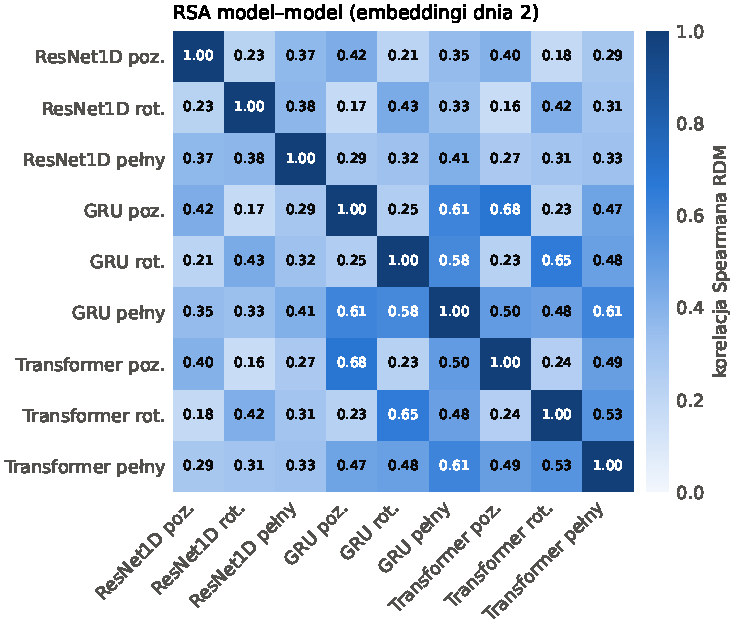
\includegraphics[width=0.72\linewidth]{rsa_models.pdf}
\caption{S3: RSA model--model (korelacja Spearmana RDM-ów, dzień 2, seed 42).}
\label{fig:rsa}
\end{figure}

\begin{itemize}
  \item \textbf{Modalność dominuje nad architekturą.} Reprezentacje są podobne przede wszystkim w
        obrębie tej samej modalności (GRU vs Transformer: pozycja 0{,}68, rotacja 0{,}65), a pozycja
        i rotacja dają różne geometrie (0{,}16--0{,}25). Modele uczą się więc w dużej mierze tej
        samej struktury, wyznaczonej przez dane wejściowe.
  \item \textbf{GRU i Transformer są sobie bliższe niż ResNet1D}: ResNet1D pełny ma korelację
        0{,}27--0{,}41 ze wszystkimi przebiegami; GRU i Transformer pełne 0{,}61.
  \item \textbf{RSA z tożsamością} odtwarza ranking z ablacji: pełny $\geq$ rotacja $>$ pozycja
        dla każdego modelu.
  \item \textbf{Pozycja koduje urządzenie} wyraźnie mocniej niż rotacja (np. GRU 0{,}087 vs 0{,}029,
        Transformer 0{,}048 vs 0{,}005) -- położenie zależy od układu współrzędnych i kalibracji
        danego zestawu, orientacja w znacznie mniejszym stopniu. GRU najmocniej koduje urządzenie i
        jednocześnie ma najniższy Rank-1: część pojemności reprezentacji zużywa na cechę
        nieistotną biometrycznie.
\end{itemize}

%=====================================================================
\subsection{S4: scenariusz rozszerzony -- w stronę SOTA}\label{sec:sota}
%=====================================================================
Scenariusze S1--S3 używają klasyfikatora uczonego entropią krzyżową, a decyzję biometryczną
podejmują na podobieństwie cosinusowym embeddingów. Te dwa cele nie są ze sobą zgodne: entropia
krzyżowa nie wymusza, by próbki tej samej osoby leżały blisko na sferze. W S4 sprawdzamy, ile
można zyskać, dopasowując trening do sposobu oceny i do zmiany dnia.

\paragraph{Protokół bez wycieku informacji z testu.} Przy doborze przepisu musimy patrzeć na wyniki
cross-day, ale nie możemy tego robić na zbiorze, na którym raportujemy wynik. Dlatego dzień~2
dzielimy po numerze rzutu: rzuty 0--4 każdej osoby na każdym urządzeniu tworzą zbiór \emph{dev}
(615 prób), a rzuty 5--9 zbiór \emph{test} (615 prób). Każda osoba i każde urządzenie występują w obu
połowach. Wszystkie decyzje (tab.~\ref{tab:sota-comp}, \ref{tab:sota-extra}) podejmujemy wyłącznie
na dev; \textbf{wynikiem S4 jest test}. Dla porównania z S1/S2 podajemy też wynik na całym dniu~2,
który jest nieco optymistyczny, bo zawiera dev.

\paragraph{Składniki przepisu.}
\begin{enumerate}
  \item \textbf{ArcFace} \cite{arcface} -- addytywny margines kątowy: logit prawdziwej klasy to
        $s\cos(\theta_y + m)$, pozostałych $s\cos\theta_j$, gdzie $\theta$ to kąt między
        znormalizowanym embeddingiem a wektorem klasy ($s = 30$, $m = 0{,}3$). Funkcja straty
        bezpośrednio optymalizuje separację kątową, czyli dokładnie to, co mierzy podobieństwo
        cosinusowe. Głowicę embeddingu zmieniamy na \code{Linear}~$\to$~\code{BatchNorm} (bez ReLU),
        żeby embedding mógł wykorzystać całą sferę.
  \item \textbf{Augmentacje} (na GPU, w jednostkach znormalizowanych): losowe przycięcie i
        rozciągnięcie w czasie (skala $\mathcal{U}(0{,}85; 1)$, czyli zmiana tempa rzutu),
        skalowanie amplitudy kanałów ($\mathcal{N}(1; 0{,}05)$) i szum gaussowski ($\sigma = 0{,}03$).
  \item \textbf{EMA wag} \cite{ema} (zanik 0{,}995 na krok); embeddingi liczymy modelem uśrednionym.
  \item \textbf{Centrowanie poziome} -- od współrzędnych $x, z$ odejmujemy ich średnią po czasie i
        sensorach w danym rzucie. Usuwa to miejsce, w którym osoba stała w danej sesji, a zachowuje
        wzrost ($y$) i wzajemne położenie hełmu i kontrolerów.
  \item \textbf{Prędkości} -- do 27 kanałów dokładamy ich pierwsze różnice w czasie (54 kanały).
        Prędkość jest niezmiennicza względem stałego przesunięcia i bezpośrednio opisuje dynamikę
        ruchu.
  \item \textbf{Harmonogram} -- 150 epok, AdamW (lr $10^{-3}$, wd 0{,}05), batch 64, 5 epok rozgrzewki
        i spadek cosinusowy do zera, bez wczesnego zatrzymania. Zbiór walidacyjny nie jest więc
        potrzebny, co pozwala trenować na \textbf{całym dniu~1} (1230 zamiast 984 próbek); galerią
        jest wtedy cały dzień~1.
  \item \textbf{InceptionTime} jako czwarty model oraz \textbf{ensemble}: konkatenacja
        znormalizowanych embeddingów modeli, co jest równoważne uśrednieniu ich podobieństw
        cosinusowych.
\end{enumerate}
Architektury ResNet1D, GRU i Transformera pozostają takie jak w S1 (tab.~\ref{tab:hparams}).

\paragraph{Ablacja składników (dev).} Tabela~\ref{tab:sota-comp} i rys.~\ref{fig:sota-comp}
pokazują efekt dokładania kolejnych składników (średnia z 2 seedów). Wiersz \emph{baseline} to ten
sam trening co w S1, ale w nowej pętli (150 epok, bez wczesnego zatrzymania).

\begin{table}[H]
\centering\small
\setlength{\tabcolsep}{4pt}
\caption{S4: ablacja składników na zbiorze dev (dzień 2, rzuty 0--4), średnia z seedów 42 i 43.
Każdy wiersz zawiera wszystkie składniki z wierszy powyżej; \emph{baseline} -- CE i cechy jak w S1,
150 epok bez wczesnego zatrzymania.}
\label{tab:sota-comp}
\begin{tabular}{@{}lrrrrrrrr@{}}
\toprule
& \multicolumn{2}{c}{ResNet1D} & \multicolumn{2}{c}{GRU} & \multicolumn{2}{c}{Transformer} & \multicolumn{2}{c}{InceptionTime} \\
\cmidrule(lr){2-3}\cmidrule(lr){4-5}\cmidrule(lr){6-7}\cmidrule(l){8-9}
Wariant & R-1 & EER & R-1 & EER & R-1 & EER & R-1 & EER \\
\midrule
\tabinput{tables/sota_components.tex}
\bottomrule
\end{tabular}
\end{table}

\begin{figure}[H]
\centering
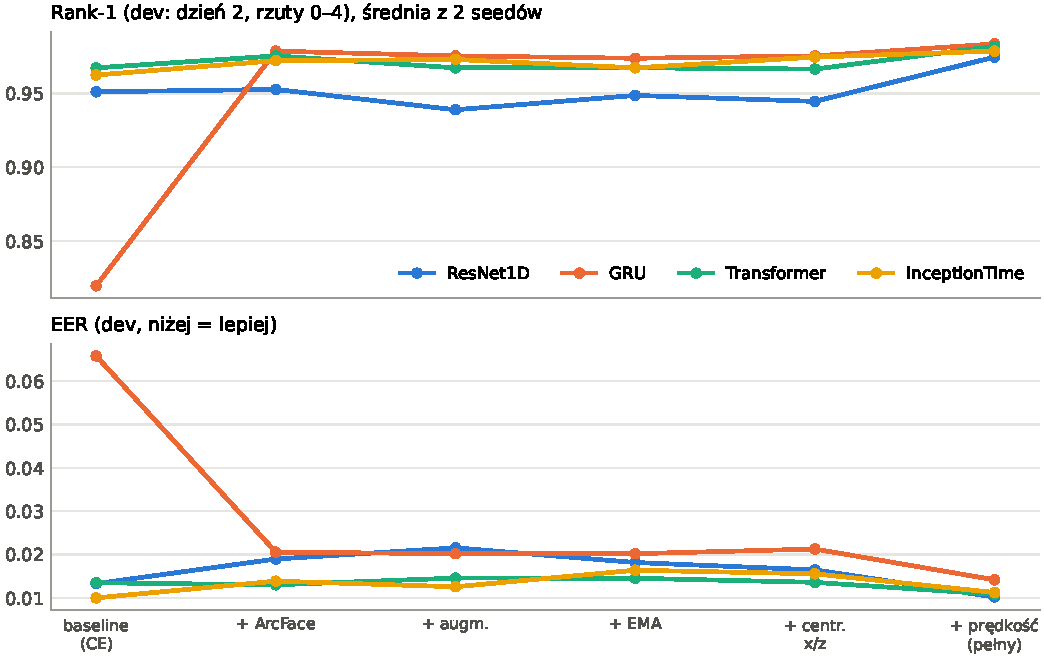
\includegraphics[width=\linewidth]{sota_components.pdf}
\caption{S4: wpływ kolejnych składników na Rank-1 i EER (dev).}
\label{fig:sota-comp}
\end{figure}

\begin{table}[H]
\centering\small
\caption{S4: pojedyncze zmiany względem pełnego przepisu (dev). GRU -- średnia z 2 seedów,
Transformer -- seed 42 (wiersz odniesienia: średnia z 2 seedów).}
\label{tab:sota-extra}
\begin{tabular}{@{}lrrrr@{}}
\toprule
& \multicolumn{2}{c}{GRU} & \multicolumn{2}{c}{Transformer} \\
\cmidrule(lr){2-3}\cmidrule(l){4-5}
Wariant & R-1 & EER & R-1 & EER \\
\midrule
\tabinput{tables/sota_extras.tex}
\bottomrule
\end{tabular}
\end{table}

\paragraph{Co działa, a co nie.}
\begin{itemize}
  \item \textbf{ArcFace} daje największy pojedynczy zysk tam, gdzie baseline był najsłabszy:
        Rank-1 GRU na dev rośnie z 0{,}820 do 0{,}979, a EER spada ponad trzykrotnie. Usunięcie ArcFace z
        pełnego przepisu (CE zamiast ArcFace) cofa GRU do 0{,}907 (tab.~\ref{tab:sota-extra}).
        Dla Transformera i InceptionTime zysk wynosi ok.~1~p.p., a dla ResNet1D jest w granicach
        szumu.
  \item \textbf{Prędkości} to drugi kluczowy składnik. Poprawiają \emph{wszystkie} cztery modele
        (ResNet1D 0{,}945~$\to$~0{,}975, Transformer 0{,}967~$\to$~0{,}982) i obniżają EER do
        ok.~0{,}010--0{,}014. Pierwsza różnica jest niezmiennicza względem stałego przesunięcia, więc
        uwypukla dynamikę ruchu, która jest stabilniejsza między dniami niż położenie.
  \item \textbf{Augmentacje, EMA i centrowanie poziome} nie dały mierzalnego zysku: zmiany mieszczą
        się w $\pm 1{,}5$~p.p., czyli do ok.~9 prób z 615 na dev (dla ResNet1D augmentacje nawet
        nieco szkodzą), a usunięcie augmentacji lub centrowania z pełnego przepisu niczego nie
        pogarsza. Zostawiamy je w przepisie, bo tak został wybrany, ale
        uczciwie raportujemy, że nie są źródłem poprawy.
  \item \textbf{Trening na całym dniu~1} poprawił dev dla obu sprawdzonych modeli (GRU
        0{,}984~$\to$~0{,}987, Transformer 0{,}982~$\to$~0{,}985), dlatego jest częścią przepisu
        finalnego. Pozostałe warianty (margines 0{,}5, skala 64, 250 epok) nie dały spójnej poprawy
        Rank-1 na obu modelach.
\end{itemize}

\paragraph{Wynik końcowy.} Przepis \emph{pełny + trening na całym dniu~1} uruchomiliśmy dla 4 modeli i
3 seedów (42, 43, 44). Ensemble wszystkich czterech modeli wybraliśmy na dev (0{,}992 wobec 0{,}991
bez GRU). Wyniki zawiera tabela~\ref{tab:sota-final}.

\begin{table}[H]
\centering\footnotesize
\setlength{\tabcolsep}{2.2pt}
\caption{S4: wynik końcowy, średnia $\pm$ odch. std. z 3 seedów. \emph{Test} -- dzień 2, rzuty 5--9,
niewidziane przy żadnej decyzji (wynik główny). Kolumna S2 -- baseline (pełny, 3 seedy) na całym
dniu 2. Galerią w S4 jest cały dzień 1.}
\label{tab:sota-final}
\begin{tabular}{@{}lrrrrrrrr@{}}
\toprule
& S2 & cały dz. 2 & \multicolumn{3}{c}{Test (dzień 2, rzuty 5--9)} & \multicolumn{3}{c}{Test: R-1 wg urządz.} \\
\cmidrule(lr){3-3}\cmidrule(lr){4-6}\cmidrule(l){7-9}
Model & Rank-1 & Rank-1 & Rank-1 & Rank-5 & EER & Quest & Vive & Cosmos \\
\midrule
\tabinput{tables/sota_final.tex}
\bottomrule
\end{tabular}
\end{table}

\begin{figure}[H]
\centering
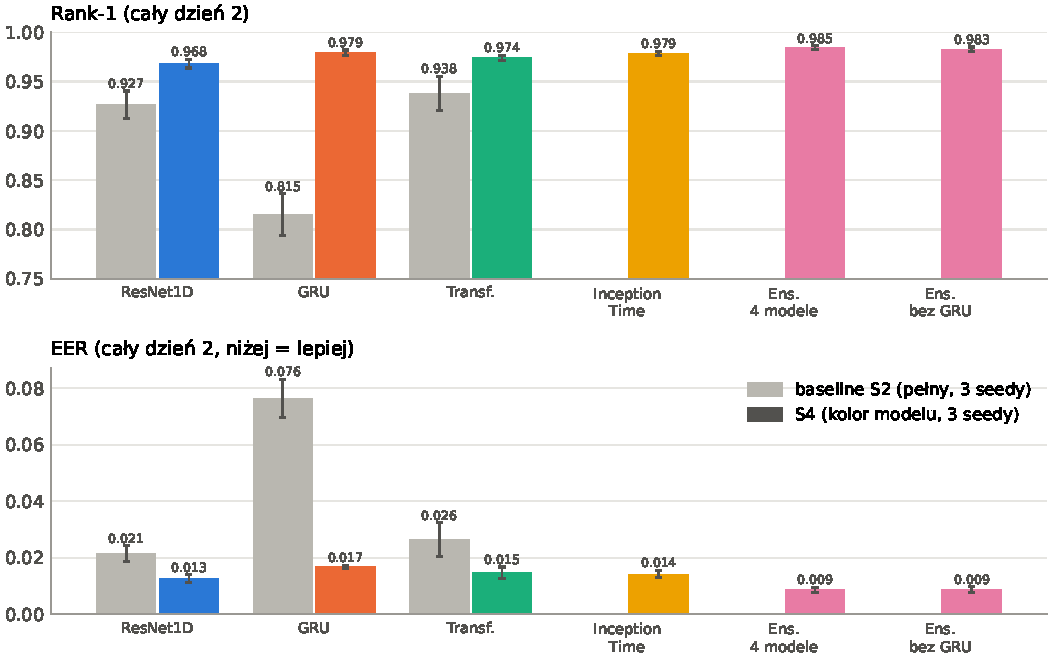
\includegraphics[width=\linewidth]{sota_vs_baseline.pdf}
\caption{S4 a baseline z S2 na całym dniu 2 (średnia $\pm$ odch. std. z 3 seedów). InceptionTime i
ensemble nie mają odpowiednika w S2.}
\label{fig:sota-vs-base}
\end{figure}

\begin{itemize}
  \item \textbf{Ensemble 4 modeli: Rank-1 $0{,}977 \pm 0{,}002$ i EER $0{,}012$ na odłożonym teście}
        (na całym dniu~2: 0{,}985 i 0{,}009). Najlepszy baseline (Transformer, 0{,}938) mylił się w
        6{,}2\% prób dnia~2, a ensemble w 1{,}5\%, czyli ok.~4 razy rzadziej. EER spadł z 0{,}021
        (najlepszy w S2) do 0{,}009.
  \item \textbf{Pojedyncze modele zbliżyły się do siebie.} Na teście wszystkie cztery mieszczą się w
        przedziale 0{,}960--0{,}972. GRU, najsłabszy w S1--S2 (0{,}815), w S4 jest wśród najlepszych
        (0{,}971): jego słabość wynikała z funkcji straty i cech wejściowych, a nie z architektury.
        Najlepszym pojedynczym modelem jest InceptionTime (0{,}972), a najniższy EER ma ResNet1D
        (0{,}016).
  \item \textbf{Geometria embeddingów:} ArcFace przesuwa pary impostor do podobieństwa ok.~0
        (ortogonalne embeddingi; w S1 było 0{,}28--0{,}47), co dobrze widać na rozkładach
        (rys.~\ref{fig:scores-sota}).
  \item \textbf{Cosmos nadal najtrudniejszy:} 0{,}93--0{,}94 Rank-1 wobec 0{,}97--1{,}00 dla Questa i
        Vive. W teście ensemble ok.~85\% pozostałych błędów (średnio 12 z 14) to próby z Cosmosa.
  \item \textbf{Optymizm dev.} Na dev ensemble osiąga 0{,}992, na teście 0{,}977. Na modelach z S1,
        które dev nigdy nie widziały, obie połowy dnia~2 są równie trudne (różnice $\pm$1~p.p. bez
        stałego kierunku), więc ok.~1~p.p. różnicy to koszt wyboru przepisu na dev. Właśnie dlatego
        jako wynik główny podajemy odłożony test.
\end{itemize}

\begin{figure}[H]
\centering
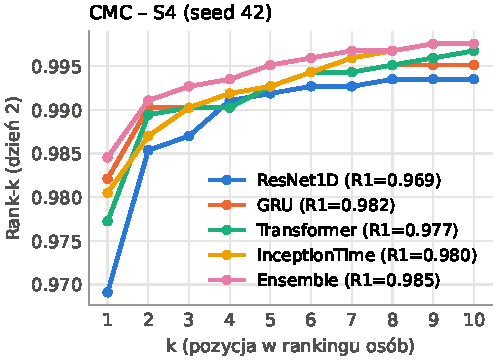
\includegraphics[width=0.55\linewidth]{cmc_sota.pdf}
\caption{S4: krzywe CMC na całym dniu 2 (seed 42). Ensemble: Rank-1 0{,}985, Rank-5 0{,}995.}
\label{fig:cmc-sota}
\end{figure}

\begin{figure}[H]
\centering
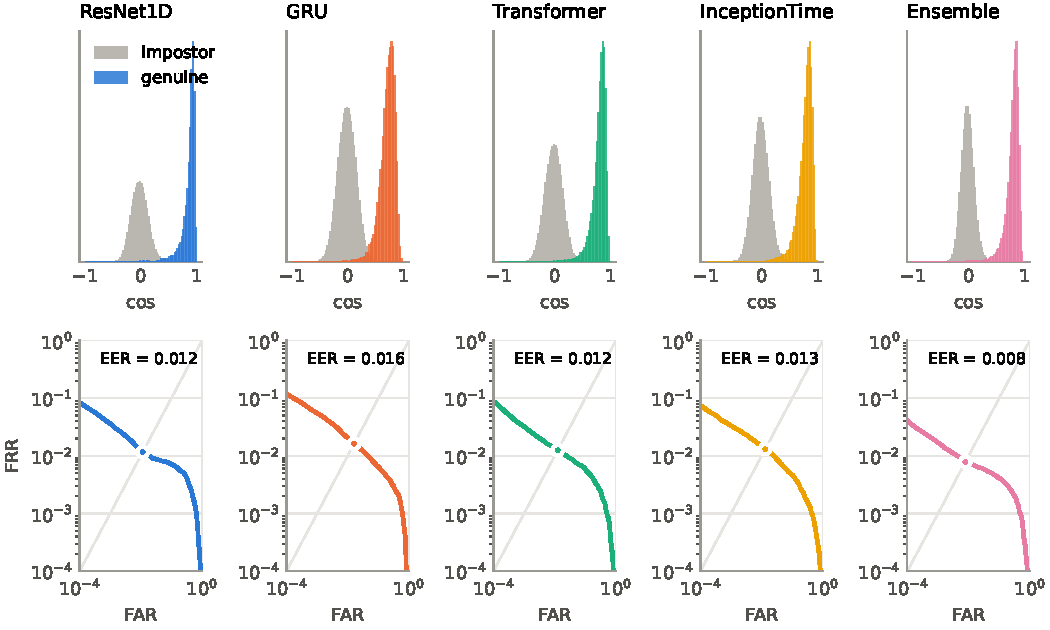
\includegraphics[width=\linewidth]{scores_sota.pdf}
\caption{S4: rozkłady podobieństwa genuine/impostor i krzywe DET (cały dzień 2, seed 42).
W porównaniu z rys.~\ref{fig:scores-base} rozkład impostor przesunął się do zera, a krzywe DET
leżą niżej.}
\label{fig:scores-sota}
\end{figure}



%=====================================================================
\section{Wnioski}\label{sec:wnioski}
%=====================================================================
\begin{enumerate}
  \item \textbf{Ruch w VR jest silną i stabilną w czasie cechą biometryczną.} Już modele bazowe
        rozpoznają osobę następnego dnia z Rank-1 0{,}93--0{,}94 (ResNet1D, Transformer), a po
        dopasowaniu treningu do oceny cosinusowej -- 0{,}977 na odłożonym teście (ensemble) przy EER
        ok.~1\%. Kształt rzutu tej samej osoby jest powtarzalny między dniami, a różnice
        międzyosobnicze (tempo, amplituda, orientacja dłoni i głowy) są wyraźne.
  \item \textbf{Reprezentacja danych waży więcej niż wybór architektury.} Dwie największe poprawy w
        projekcie nie wynikają z modelu, tylko z cech wejściowych i funkcji straty:
        (a) ciągła reprezentacja 6D rotacji zamiast kątów Eulera -- odwróciła ranking modalności i
        podniosła Rank-1 rotacji GRU z 0{,}52 do 0{,}74; (b) ArcFace i prędkości -- podniosły
        GRU z 0{,}82 do 0{,}97--0{,}98 i zrównały wszystkie cztery architektury (0{,}960--0{,}972).
        RSA prowadzi do tego samego wniosku: embeddingi różnych modeli z tej samej modalności są do
        siebie bardziej podobne niż embeddingi jednego modelu z różnych modalności.
  \item \textbf{Modalności:} pełny $>$ rotacja $>$ pozycja dla każdego modelu i każdej metryki.
        Rotacja (orientacja kontrolerów i hełmu) niesie więcej informacji biometrycznej niż pozycja,
        a obie są komplementarne. Pozycja dodatkowo koduje urządzenie (RSA z urządzeniem do 0{,}09),
        czyli cechę niepożądaną w biometrii.
  \item \textbf{Urządzenia:} najwięcej informacji biometrycznej dostarcza Quest (najwyższy Rank-1 w
        9/9 konfiguracjach S2), potem Vive; najmniej -- Cosmos (najniższy Rank-1 w 9/9 konfiguracjach
        S2 i we wszystkich modelach S4; w S4 to 0{,}93--0{,}94 wobec 0{,}97--1{,}00). Większość
        błędów najlepszego systemu pochodzi z Cosmosa.
  \item \textbf{Porównanie klasyfikatorów.} W ustawieniu bazowym (CE): Transformer $\geq$ ResNet1D
        $\gg$ GRU. Transformer najlepiej separuje osoby przy 6 razy mniejszej liczbie parametrów niż
        ResNet1D, a GRU jest najsłabszy i najmocniej koduje urządzenie. W ustawieniu S4 różnice
        prawie znikają, a najlepszy pojedynczy model to InceptionTime. Ensemble różnych architektur
        jest najlepszy (Rank-1 0{,}977, EER 0{,}012), bo modele mylą się na różnych próbach.
  \item \textbf{Metodologia oceny.} Walidacja w obrębie dnia~1 jest nasycona (Rank-1 0{,}97--1{,}00)
        i nie przewiduje wyniku cross-day, dlatego model wybieramy po val loss. Dobór przepisu na
        części dnia~2 zawyża wynik o ok.~1~p.p. (dev 0{,}992 vs test 0{,}977), dlatego raportujemy
        odłożony test. Ranking Rank-$k$ musi być liczony po osobach, a nie po próbkach.
\end{enumerate}

\paragraph{Ograniczenia.} 41 osób i jedno zadanie ruchowe; identyfikacja w zbiorze zamkniętym
(wszystkie osoby są w galerii); dwa dni nagrań, więc nie wiemy, jak wynik zachowuje się po
tygodniach. Przepis S4 wybieraliśmy na 2 seedach i części wariantów, a różnice rzędu
$\pm 1{,}5$~p.p. na dev (do ok.~9 prób z 615) są na granicy szumu. Hipotezy o przyczynach słabości Cosmosa
(jakość śledzenia) nie da się zweryfikować na tym korpusie.

\paragraph{Dalsze kierunki.} Weryfikacja w zbiorze otwartym (osoby spoza treningu w galerii i
próbach), adaptacja domeny między dniami, oddzielne modele lub normalizacja per urządzenie dla
Cosmosa oraz analiza, które fragmenty rzutu (np. przez mapy uwagi Transformera) niosą najwięcej
informacji biometrycznej.


%=====================================================================
\section{Odtwarzalność}\label{sec:odtwarzalnosc}
%=====================================================================
Kod (PyTorch) i wyniki są w załączonym archiwum ZIP oraz w repozytorium projektu. Wszystkie liczby
w raporcie są generowane z plików \code{results/} skryptami \code{report/make\_tables.py} i
\code{report/make\_figures.py}. Na karcie RTX 3070 Ti scenariusze S1--S3 trwają ok.~9 minut
(strojenie 2{,}5 min, trening 3 modeli 50 s, ablacja 27 przebiegów 5 min, RSA 10 s), a S4 ok.~1{,}5 h
(screening 4 modeli w 4 równoległych procesach i finał 4 modele $\times$ 3 seedy, ok.~20 min). Dane trzymamy w całości w pamięci GPU i batchujemy indeksami zamiast przez
\code{DataLoader}, co skraca epokę z ok.~17~s (CPU) do poniżej 1~s.

\begin{lstlisting}
pip install torch --index-url https://download.pytorch.org/whl/cu130
pip install -r requirements.txt
python tune_models.py --model all --trials 6 --epochs 15      # random search
python train_resnet.py --no-dashboard                          # S1 (analogicznie gru, transformer)
python ablation.py                                             # S2: 3 modele x 3 modalnosci x 3 seedy
python rsa.py                                                  # S3
python sota.py screen --models gru --variants base arcface arc_aug arc_aug_ema \
    arc_aug_ema_center full full_ce full_day1    # S4: wybor przepisu na dev (analogicznie inne modele)
python sota.py final                                           # S4: full_day1, 4 modele + 2 ensemble, 3 seedy
python report/make_tables.py && python report/make_figures.py  # tabele i wykresy raportu
python report/make_zip.py                                      # archiwum do oddania
\end{lstlisting}

Embeddingi, zgodnie z poleceniem, zapisujemy w katalogu \code{embeddings/<przebieg>/} w plikach
\code{train\_embedding.npz} oraz \code{test\_embedding.npz} (dodatkowo \code{val\_embedding.npz}). Każdy plik zawiera tablice \code{embeddings}, \code{labels} i
\code{device\_ids}. Przebiegi:
\begin{itemize}
  \item \code{resnet}, \code{gru}, \code{transformer} -- S1;
  \item \code{<model>\_position}, \code{<model>\_rotation}, \code{<model>\_full} -- S2 (wejście RSA);
  \item \code{sota\_<model>} oraz \code{sota\_ensemble\_*} -- S4.
\end{itemize}

\begin{thebibliography}{9}\small
\bibitem{dataset} weibo053, \emph{VR-Biometric-Authentication} (repozytorium danych), commit
  \code{4bbc555}, \url{https://github.com/weibo053/VR-Biometric-Authentication}.
\bibitem{zhou6d} Y.~Zhou, C.~Barnes, J.~Lu, J.~Yang, H.~Li, \emph{On the Continuity of Rotation
  Representations in Neural Networks}, CVPR 2019.
\bibitem{resnet} K.~He, X.~Zhang, S.~Ren, J.~Sun, \emph{Deep Residual Learning for Image
  Recognition}, CVPR 2016.
\bibitem{gru} K.~Cho i in., \emph{Learning Phrase Representations using RNN Encoder--Decoder for
  Statistical Machine Translation}, EMNLP 2014.
\bibitem{transformer} A.~Vaswani i in., \emph{Attention Is All You Need}, NeurIPS 2017.
\bibitem{inceptiontime} H.~Ismail Fawaz i in., \emph{InceptionTime: Finding AlexNet for Time Series
  Classification}, Data Mining and Knowledge Discovery 34, 2020.
\bibitem{arcface} J.~Deng, J.~Guo, N.~Xue, S.~Zafeiriou, \emph{ArcFace: Additive Angular Margin Loss
  for Deep Face Recognition}, CVPR 2019.
\bibitem{adamw} I.~Loshchilov, F.~Hutter, \emph{Decoupled Weight Decay Regularization}, ICLR 2019.
\bibitem{randomsearch} J.~Bergstra, Y.~Bengio, \emph{Random Search for Hyper-Parameter
  Optimization}, JMLR 13, 2012.
\bibitem{rsa} N.~Kriegeskorte, M.~Mur, P.~Bandettini, \emph{Representational Similarity Analysis --
  Connecting the Branches of Systems Neuroscience}, Frontiers in Systems Neuroscience, 2008.
\bibitem{ema} B.~T.~Polyak, A.~B.~Juditsky, \emph{Acceleration of Stochastic Approximation by
  Averaging}, SIAM J. Control and Optimization 30(4), 1992.
\end{thebibliography}

\end{document}
